\section{Experimental site and Instrumentation}\label{sec:site_instruments_products}

The AGORA ACTRIS-CCRES station (37$^{\circ}$2'E, 3$^{\circ}$6'S, 680 masl) is located in the Southern of the Iberian Peninsula being one the most meridional CLOUDNET stations. This station is marked by colder months during winter and spring and warm months during summer and fall. Especially between summer and winter, the changes in temperature and humidity are strictly high at this station, as revealed by \cite{andresestebanbedoya-velasquezSeasonalAnalysisAtmosphere2019}. The authors show that these changes are mainly due to solar incidence, being the diurnal cycle a strong component in seasonal differences. For non cloudy data, typically surface temperature in summer can vary around 30 – 40 $^{\circ}$C, meanwhile they vary around 15 $^{\circ}$C in winter at 16 UTC. For the same time, the relative humidity below 5 km a.g.l presented the opposite behavior, with maximum found between 2 and 10 UTC, and from 9 UTC to midnight. This maximum can range between 60-75\% during winter, and 40-50\% during summer. However, larger values were also detected above 5 km at 16 UTC within thinner layers for all seasons. The height of this humidity layer can vary with seasons, being higher in summer and fall (7-9 km) and lower in winter and spring (5-7 km). These thermodynamic conditions will be particularly important to understand diurnal cycle of cloud types and inter-annual differences in cloud properties analyzed in further sections.

\subsubsection{Instrumentation}

In this study we use a combination of active and passive remote sensors that are part of ACTRIS CCRES and exploited in CLOUDNET. These instruments include a MWR, a ceilometer and a cloud radar. An overview of each instrument is provided next.
The RPG-HATPRO G2 (Humidity and Temperature PROfiler) is a passive remote sensing instrument that measures the brightness temperature around the water vapor (22-31 GHz) and oxygen (51-58 GHz) absorption bands. This instrument has radiometric accuracy of 0.3-0.4 K and provides accurate values of retrieved liquid water path (LWP) and integrated water vapor (IWV) with 1\,s of integration time \citep{lohnertAccuracyCloudLiquid2003}. In addition, its dual-channel system makes it possible to provide temperature and humidity profiles with the same time resolution. 

The CHM15k Nimbus ceilometer is an active remote sensing instrument that works with a pulsed laser of Nd:YAG. It measures in the photon-counting mode and provides the  attenuated backscattering coefficient ($\beta$) of aerosols and small cloud droplets. This instrument has repetition frequency range about  5-7 kHz, where each pulse is emitted at 1064 nm with 8.4 $\mu$J of energy. The laser beam has a range resolution of 15 m and can diverge 0.3 mrad, reaching a complete overlap of about 1500m a.g.l \cite{heeseCeilometerLidarComparison2010}. Especifically, this ceilometer is operated with a time resolution of 15\,s.

The dual polarimetric RPG-FMCW 94 GHz Doppler cloud radar is also an active remote sensing instrument that operates at 94 GHz. This instrument uses the frequency-modulated continuous wave (FMCW) signal which makes it possible to vary the vertical and temporal resolution. Their frequency range is from 300-3700 kHz and the antenna beam width is 0.56 $^{\circ}$. 
It measures the Doppler velocity spectrum (DVS) for horizontal and vertical linear polarizations at 94 GHz. Unlike traditional single polarization measurements that retrieve only reflectivity (Z), mean Doppler velocity (ν$_{D}$), and spectral width (S$_{\omega}$), this advanced radar also derives the linear depolarization ratio (LDR), enabling the detection of the melting layer, aerosols, and insects as described by \cite{hoganFacilitatingCloudRadar}.
Table \ref{tab:info_instrument} provides an overview of the AGORA instrumentation, detailing operational frequencies or wavelengths, type of measurements, products, measurement ranges, data collection intervals, and references with detailed descriptions.

\begin{table}[H]
	\caption{Summary of instruments and their data products. }
	\begin{tabular}{@{}lllllll@{}}
		\toprule
		\textbf{Instrument}                                                         & \textbf{Bands / wavelengths}                                                                     & \textbf{Measured}                                                                   & \textbf{Products}                                          & \textbf{Range}                                                                           & \textbf{Time}                                                                           & \textbf{References}                         \\ \midrule
		\begin{tabular}[c]{@{}l@{}}94 GHz Cloud \\ Doppler Radar\end{tabular}       & 94 GHz (W-band)                                                                                  & \begin{tabular}[c]{@{}l@{}}Doppler velocity \\ spectrum (DVS)\end{tabular}          &  $\nu_{D}$ , Z, S$_{w}$ & [13,51]\,m \tnote{a} & [1.1, 3.6]\,s \tnote{b}  & \cite{nilskuchlerWBandRadarRadiometer2017}                               \\
		\hline
		&                                                                                                  &                                                                                     & q and T                                                    & [10, 300]\,m \tnote{c}       & [2, 2.5]\,min                                                                             &                                             \\ 
		\multirow{-2}{*}{\begin{tabular}[c]{@{}l@{}}MWR RPG \\ HATPRO\end{tabular}} & \multirow{-2}{*}{\begin{tabular}[c]{@{}l@{}}22-31 GHz (K-band)\\ 51-58 GHz (V-band)\end{tabular}} & \multirow{-2}{*}{\begin{tabular}[c]{@{}l@{}}Brightness \\ Temperature\end{tabular}} & LWP                                                        & -                                                                                        & 2 s                                                                                     & \multirow{-2}{*}{\cite{francisconavas-guzmanTroposphericWaterVapour2014}} \\
		\hline
		\begin{tabular}[c]{@{}l@{}}CHM15k \\ Nimbus \\ Ceilometer\end{tabular}      & 1064 nm                                                                                          &                                                                                     & $\beta$                              & 15 m                                                                                     & 15 s                                                                                    & \cite{a.cazorlaNearrealtimeProcessingCeilometer2017}                      \\ \bottomrule
	\end{tabular}
	\label{tab:info_instrument}
	\begin{tablenotes}
		\footnotesize
		\item[a] This range varies with the height and depends on the chirp table configuration.
		\item[b] It also depends on the chirp type.
		\item[c] Humidity and temperature profiles have a range varying from 10 to 150 m in the first 4.4 km and from 50 to 300 m between 4.4 and 10 km.
	\end{tablenotes}
\end{table}

Overall, a synergistic combination of these instruments have been widely used for many cloud remote sensing stations as part of the Cloudnet consortium. This combination shows a promising configuration for long-term cloud observations \citep{j.a.ContinuousEvaluationCloud2007}, especially to calculate cloud microphysics. Particularly, ground-based radar measurements can be used to retrieve cloud microphysics with better accuracy than satellites \citep{protatAssessmentCloudsatReflectivity2009}.

\section{Cloudnet database}

%%%%%%%%%%%%%%%%%%%%%%%%%%%
% Información cloudnet de la introducción
%%%%%%%%%%%%%%%%%%%%%%%%%%%

In order to improve cloud analysis, the AGORA station has been part of Cloudnet since 2018 and was integrated into ACTRIS CCRES (where ACTRIS stands for Aerosols, Clouds, and Trace gasses Research InfraStructure, and CCRES for Centre for Cloud Remote Sensing) in 2023 as a new facility. The Cloudnet processing chain \citep{j.a.ContinuousEvaluationCloud2007} performs extensive quality assurance on raw instruments for providing high-level products, such as target classification, liquid water path, and droplet effective radius. This chain standardizes data processing within the cloud remote sensing community. Their products are derived using a synergistic approach, integrating vertically pointing measurements from ground-based instruments like Doppler cloud radars, microwave radiometers, and ceilometers. Specifically, the target classification product, generated through these three instruments, has been utilized in numerous studies for cloud typing and multi-year analysis \citep{razvanpirloagaGroundBasedMeasurementsCloud2022, tatiananomokonovaStatisticsCloudsTheir2019, stefankneifelMultiyearCloudPrecipitation2021}.
Therefore, an extensive dataset spanning the years 2018 to 2023 was utilized in this study.
Figure \ref{fig:data_availability} illustrates the monthly Cloudnet high level products availability for the AGORA ACTRIS-CCRES station. The availability of this data depends on simultaneous vertically pointing measurements of the microwave radiometer, ceilometer, Doppler cloud radar, as well as the meteorological model products - the ECMWF model (European Centre for Medium-Range Weather Forecasts). As observed, the months with lower data availability are Jan-Mar, with 40-50\% of the data available, whereas from Apr to Oct the data availability is over 60\% .The years 2018 (270,000 profiles) and 2020 (968,769 profiles) are the years with the least and greatest amount of data. The white bars denote periods with missing data due to instrument maintenance, technical issues, and scanning measurements. Despite the missing periods, the recorded dataset establishes a solid database, covering more than 50% of all these six years.

\begin{figure}[H]
	\centering
	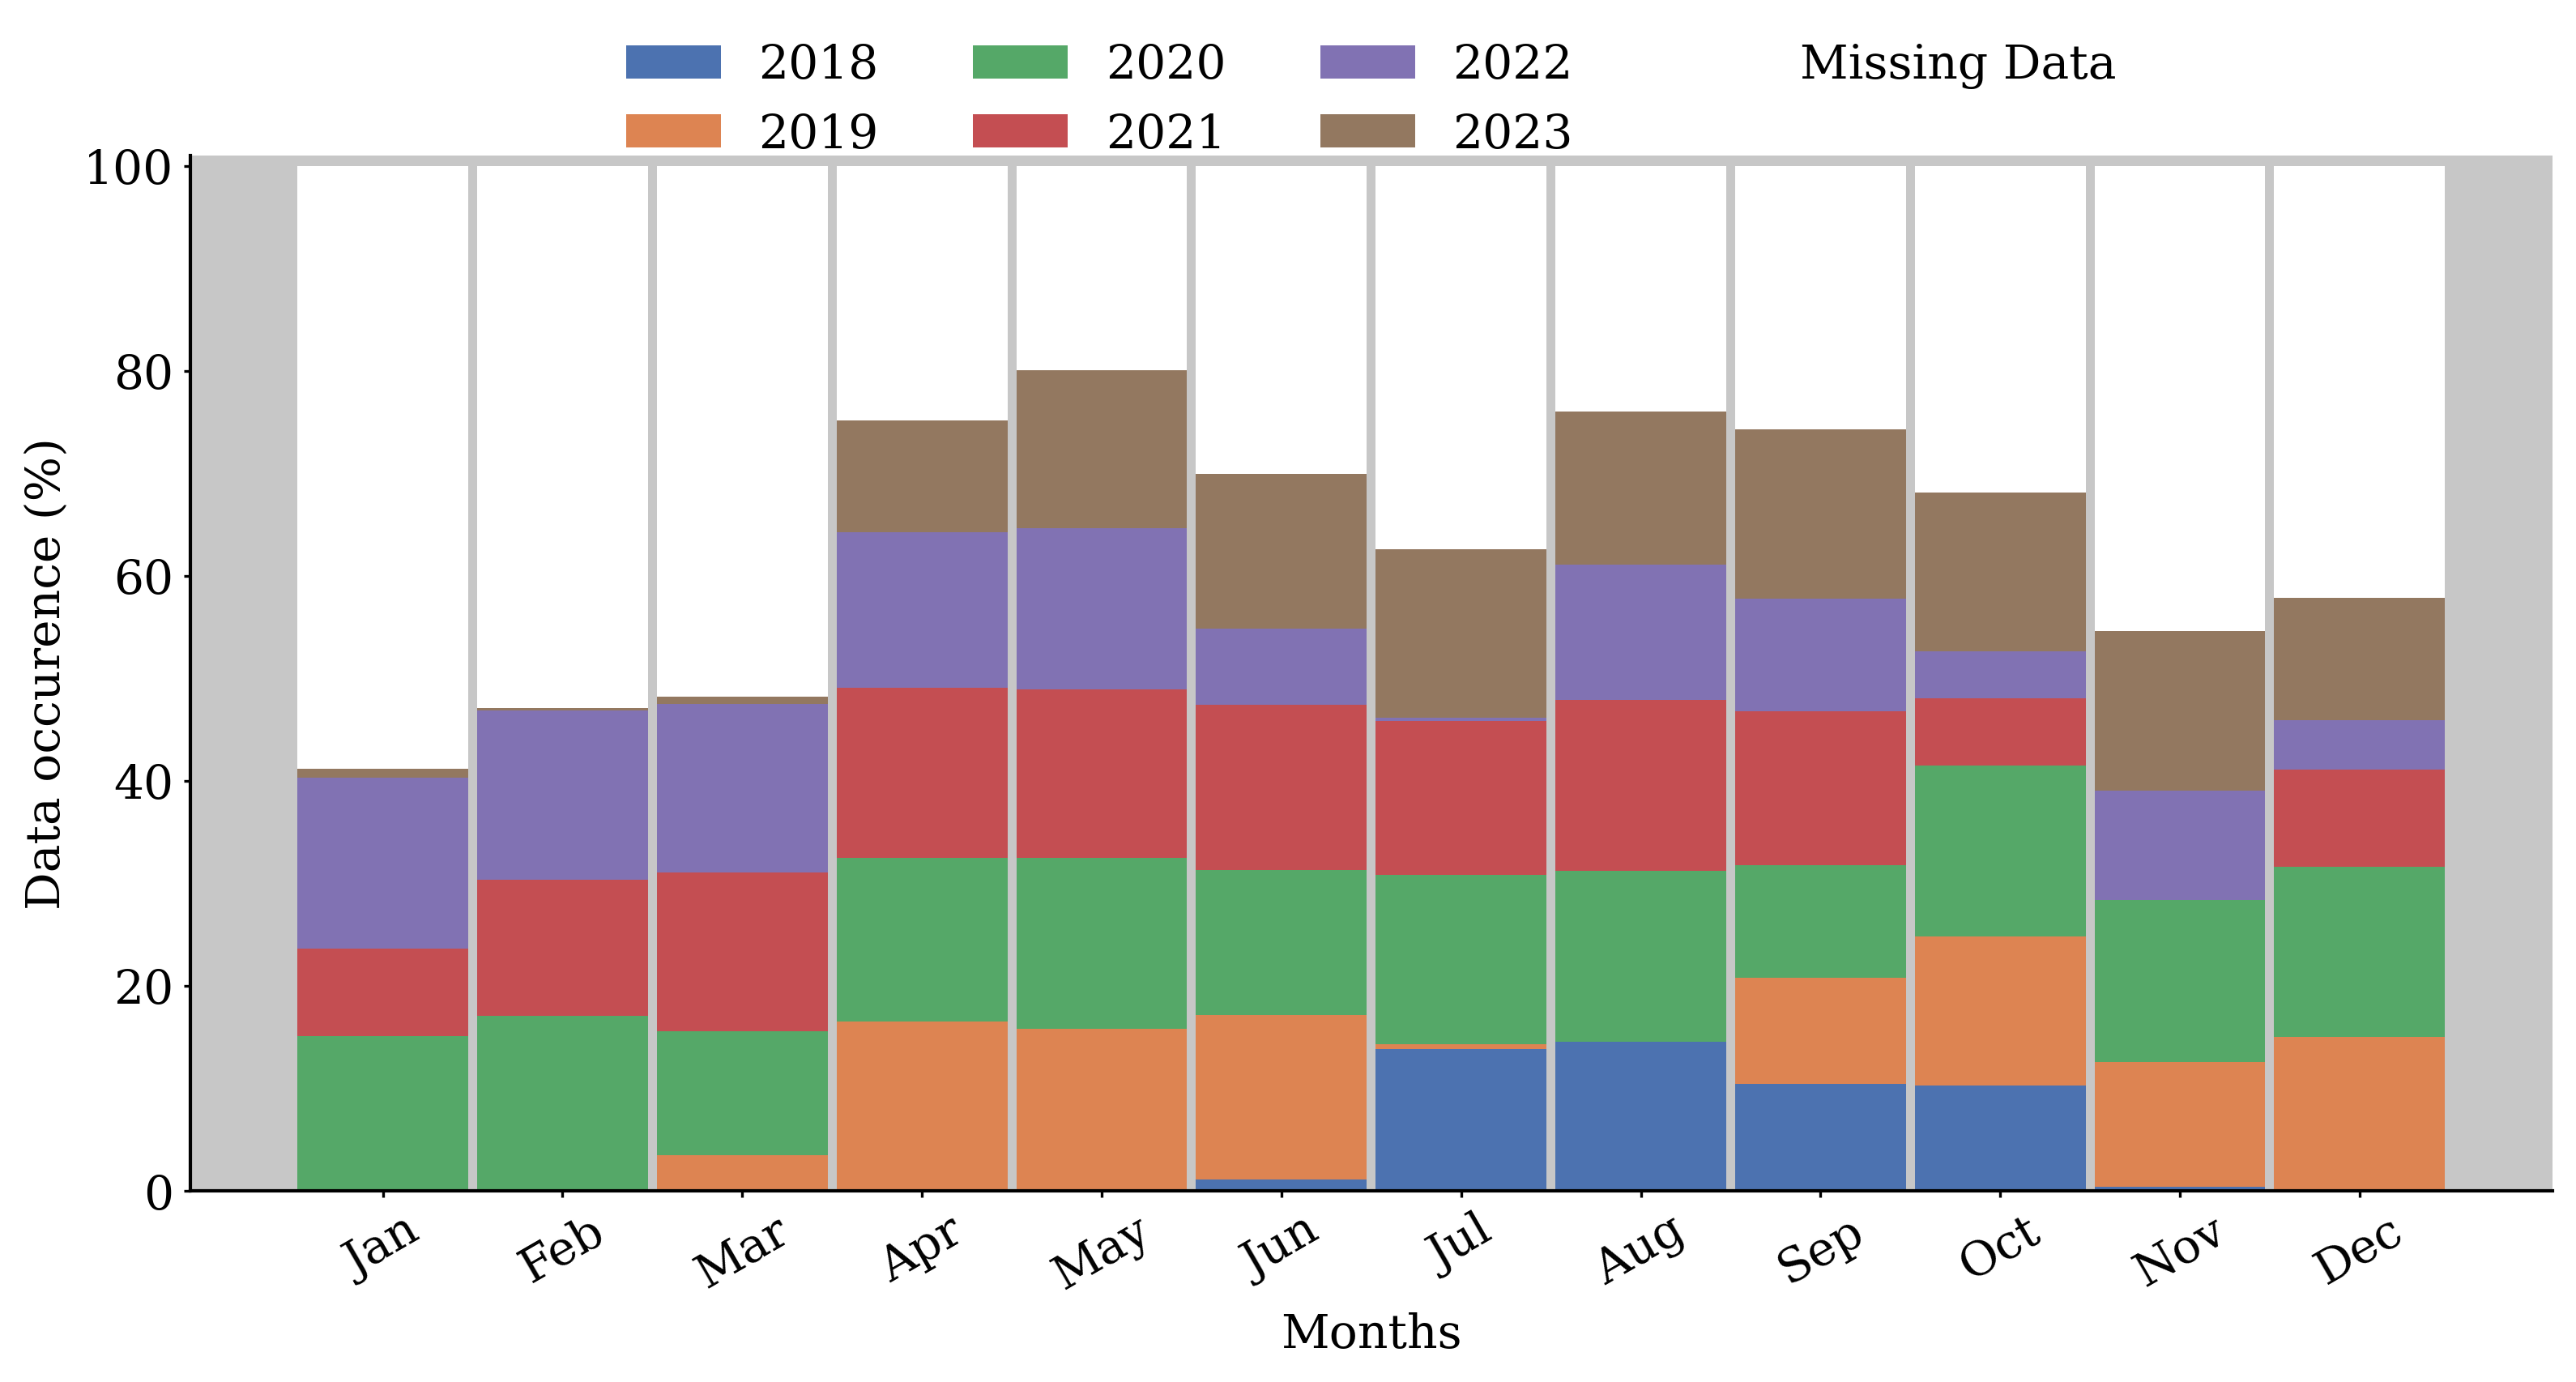
\includegraphics[width=.8\textwidth]{../../phd_clouds/figures/new_method_separated_monthly_data_occurence}
	\caption{High level post-processed data availability per month at the AGORA ACTRIS CCRES station. This dataset represents more than half a decade of synergic ground-based measurements at this station. Each color represents the data availability for different years.}
	\label{fig:data_availability}
\end{figure}

\subsubsection{Data processing}\label{sec:cloudnet_products}

Instrument datasets are processed by Cloudnet processing chain \citep{j.a.ContinuousEvaluationCloud2007} as follows:
\begin{enumerate}
	\item Set a common grid with a temporal resolution of 30\,s and spatial resolution according to the radar (see table \ref{tab:info_instrument}), respectively. It should be noted that this Cloudnet grid difficulties the monthly profiling on cloud statistics. Hence, another regrinding interpolating onto a height resolution of 20\,m is applied in the microphysics analysis.
	
	\item Corrections: this includes two-way gas and liquid reflectivity attenuation, error estimation, and quality flag assignment. High-frequency radars experience significant attenuation from gas and liquid droplets, necessitating signal correction. This issue is particularly pronounced during heavy rain events, where liquid layers on radome sheets can cause an attenuation of 14 dB \cite{hoganAbsoluteCalibration942003}.
	
	\item Cloud boundaries determination: lidar attenuated backscatter coefficient ($\beta$), and radar reflectivity are used. The first is sensitive to small liquid droplets present in cloud bases, as the second are able to penetrate clouds and detect their tops.
	
	\item Target classification product: This product classifies atmospheric particles into different categories by assigning an integer ranging from 0 to 10 at each pixel in the Cloudnet processed grid. Categorizes are as follows: Clear sky (0), Droplets (1), Drizzle or rain (2), Drizzle \& droplets (3), Ice (4), Ice \& droplets (5), Melting ice (6), Melting \& droplets (7), Aerosol (8), Insects (9), Aerosol \& insect (10). These targets were determined through radar and lidar variables in combination with thermodynamic profiles from the ECMWF model. In particular, wet bulb temperature (T$_w$) profiles are used to determine the 0$^{\circ}$C isotherm and establish warm and cold regions to identify liquid and ice hydrometeors. 
	
	\item Liquid layers respect a threshold of T < -40 $^{\circ}$C, since it is not possible to keep water in liquid phase below that temperature. Moreover, liquid droplets assigned as falling were classified as drizzle or rain droplets, where falling is attributed through radar echoes analysis once particle boundaries were already determined. Therefore, falling cold particles were just classified as ice, without distinguishing ice from precipitating ice.
	
	\item Melting layers were identified at the height of maximum wet bulb temperature divergence. Pixels with divergence surpassing 0.0075 s$^{-1}$ within 150 m of height deviation were also classified as "melting". Furthermore, more than one class of particle can be settled in the same pixel, allowing the identification of mixed phase hydrometeors, like ice coexisting with supercooled liquid droplets and melting ice particles coexisting with cloud liquid droplets. A more detailed description of particle apportionment of Cloudnet algorithm can be found on \citet{hoganFacilitatingCloudRadar}. 
	
	\item The liquid water content (LWC) retrieval assumes a log-normal distribution for warm cloud droplets lifting adiabatically from its base. Its relation depends on atmospheric temperature (T) and pressure (P). This method incurs a relative uncertainty of 15\% as shown by \cite{a.s.frischCloudRadarMicrowave1998}. At our station, T and P values utilized by the LWC retrieval are provided by the European Centre for Medium-Range Weather Forecasts (ECMWF). The retrieval equation is applied exclusively to liquid pixels within cloud boundaries, which are determined by Doppler radar reflectivity (Z) and ceilometer-lidar attenuated backscatter coefficient. The liquid pixels, as ice, insect and aerosol pixels are given by the cloudnet target classification product \citep{hoganFacilitatingCloudRadar}. Additionally, LWC values are scaled to align with the Liquid Water Path (LWP) derived from the microwave radiometer. The liquid cloud droplet effective radius ($r_{liq}$) is retrieved by assuming a log-normal size distribution for warm cloud droplets. This method is insensitive to droplet number concentration and the logarithmic spread of the distribution \citep{s.frischRetrievalStratusCloud2002}. Consequently, its primary source of uncertainty is the reflectivity factor error, resulting in a relative error of 15\% for $r_{liq}$ retrievals. This relationship is applied exclusively to liquid pixels, where necessary input data, assumptions, relative errors and the studies from which these products are sourced are indicated in Table \ref{tab:microphys}).
	
	\item The ice water content (IWC) retrieval employs an empirical equation as determined by \cite{robinj.hoganRetrievalIceWater2006}, known as the Z-IWC-T relation, which depends on radar reflectivity and temperature. Compared to other microphysical variables, IWC retrievals has the largest relative uncertainties. For the W-band, the relative error is +55\% to -35\% for temperatures within the range of -20$^{\circ}$C to -10$^{\circ}$C, and +90\% to -47\% for T < -40$^{\circ}$C. While temperature is a significant parameter in IWC error estimation, \cite{pablosaavedragarfiasAsymmetriesCloudMicrophysical2023} demonstrated that the primary source of uncertainty is the reflectivity factor error. A typical reflectivity error of 3\% can result in a 12\% error in the ice water path (IWP), which is the integration of IWC over the atmospheric column. Therefore, errors in IWC can be relatively large. The Z-IWC-T relation is applied only to ice pixels within cloud boundaries. Next, the ice cloud particle effective radius ($r_{ice}$) is obtained following \cite{juliendelanoeCharacterizationIceCloud2007}, who assumed the same empirical relation for IWC and the visible extinction coefficient ($\alpha$) derived by \cite{robinj.hoganRetrievalIceWater2006}. This approach, termed the Z-T relation, depends on both T and Z, and has aThis approach, termed the Z-T relation, depends on both T and Z, and has a relative uncertainty of 50\% of $r_{ice}$ \citep{hannesgriescheApplicationShipborneRemote2020}. In general, these high relative errors emphasize how challenging it is to retrieve ice properties accurately (see Table \ref{tab:microphys})
\end{enumerate}

% Please add the following required packages to your document preamble:
% \usepackage{booktabs}
% \usepackage{multirow}
\begin{table}[H]
	\caption{Cloudnet microphysics products used in this study, their inputs and assumptions}
	\begin{tabular}{@{}llll@{}}
		\toprule
		\textbf{Cloudnet products}                  & \textbf{Input role}                              & \textbf{$\sigma_{re}$/$r_{e}$} & \textbf{References}                                                                \\ \midrule
		\multirow{3}{*}{Liquid water content (LWC)} & Z and $\beta$: cloud base and top identification & \multirow{3}{*}{15\%}          & \multirow{3}{*}{Frisch et al. (1998)}                                              \\
		& T, P, assuming an adiabatic lifting          &                                &                                                                                    \\
		& MWR or CDR LWP to scale LWC                      &                                &                                                                                    \\
		Ice water content (IWC)                     & Z and T profiles                        & -35\% to 90\%                        & \begin{tabular}[c]{@{}l@{}} \cite{robinj.hoganRetrievalIceWater2006} \\ \cite{juliendelanoeCharacterizationIceCloud2007}\end{tabular} \\
		Droplet effective radius ($r_{liq}$)       & Z, and N and $\sigma$ of lognormal PSD           & 15\%                           & \cite{s.frischRetrievalStratusCloud2002}                                                               \\
		Ice effective radius ($r_{ice}$)          & Z and T                                & 50\%                        & \cite{hannesgriescheApplicationShipborneRemote2020} \\ \bottomrule
	\end{tabular}
	\label{tab:microphys}
\end{table}

\section{Methodology}\label{sec:classification_algorithm}

\subsection{Cluster classification method}\label{sec:new_method}

The cluster-based algorithm is developed in order to homogenize cloud clusters in time. Different from the profile-based method, this method avoids high correlation between distinct cloud categories (e.g. ice and mixed-phase). In both cases, the Cloudnet target classification product is used as a basis for cloud typing. This product provides the hydrometeor type information for each profile. Thus, the pixels classified as hydrometeors, such as Droplets, Ice and Drizzle \& Droplets are used to classify clouds. In the case of the profile-based method, \cite{buhlMeasuringIceLiquidwater2016} already adapted it for only mixed phase clouds, selecting only cases with more than 15 min of coherent cloud profiles (with similar cloud profiling within 300 s). Nevertheless, by adding new criterias to identify liquid and ice clouds, this method can classify segments of one cloud in different categories, depending on the time threshold. Hence, we introduce a new approach that does not classify cloud profiles neither segments, but cloud clusters.

Prior to the use of the target classification product, a preprocessing of the data was required. It has been observed that for some specific cases, misclassification of some pixels may occur. Figure \ref{fig:cloudnet_misclassification} illustrates a thinner and lower precipitable ice cloud present between 08:00 and 20:00. However, there is no evidence of clouds in the attenuated backscatter and the radar reflectivity. These misclassifications stem from an inaccurate representation of the temperature profile by the models in the region of Granada, affecting the target classification algorithm, and subsequently, the cloud classification performed in this study. To mitigate these issues and prevent misinterpretation of future cloud statistics, we established a filter to detect and remove these cases. Basically, all these clouds which were identified with mean cloud base below 4 km (above mean sea level) and average cloud thickness below 700 meters were reclassified as noise. These values were determined empirically by studying many cases separately. 

\begin{figure}[H]
	\centering
	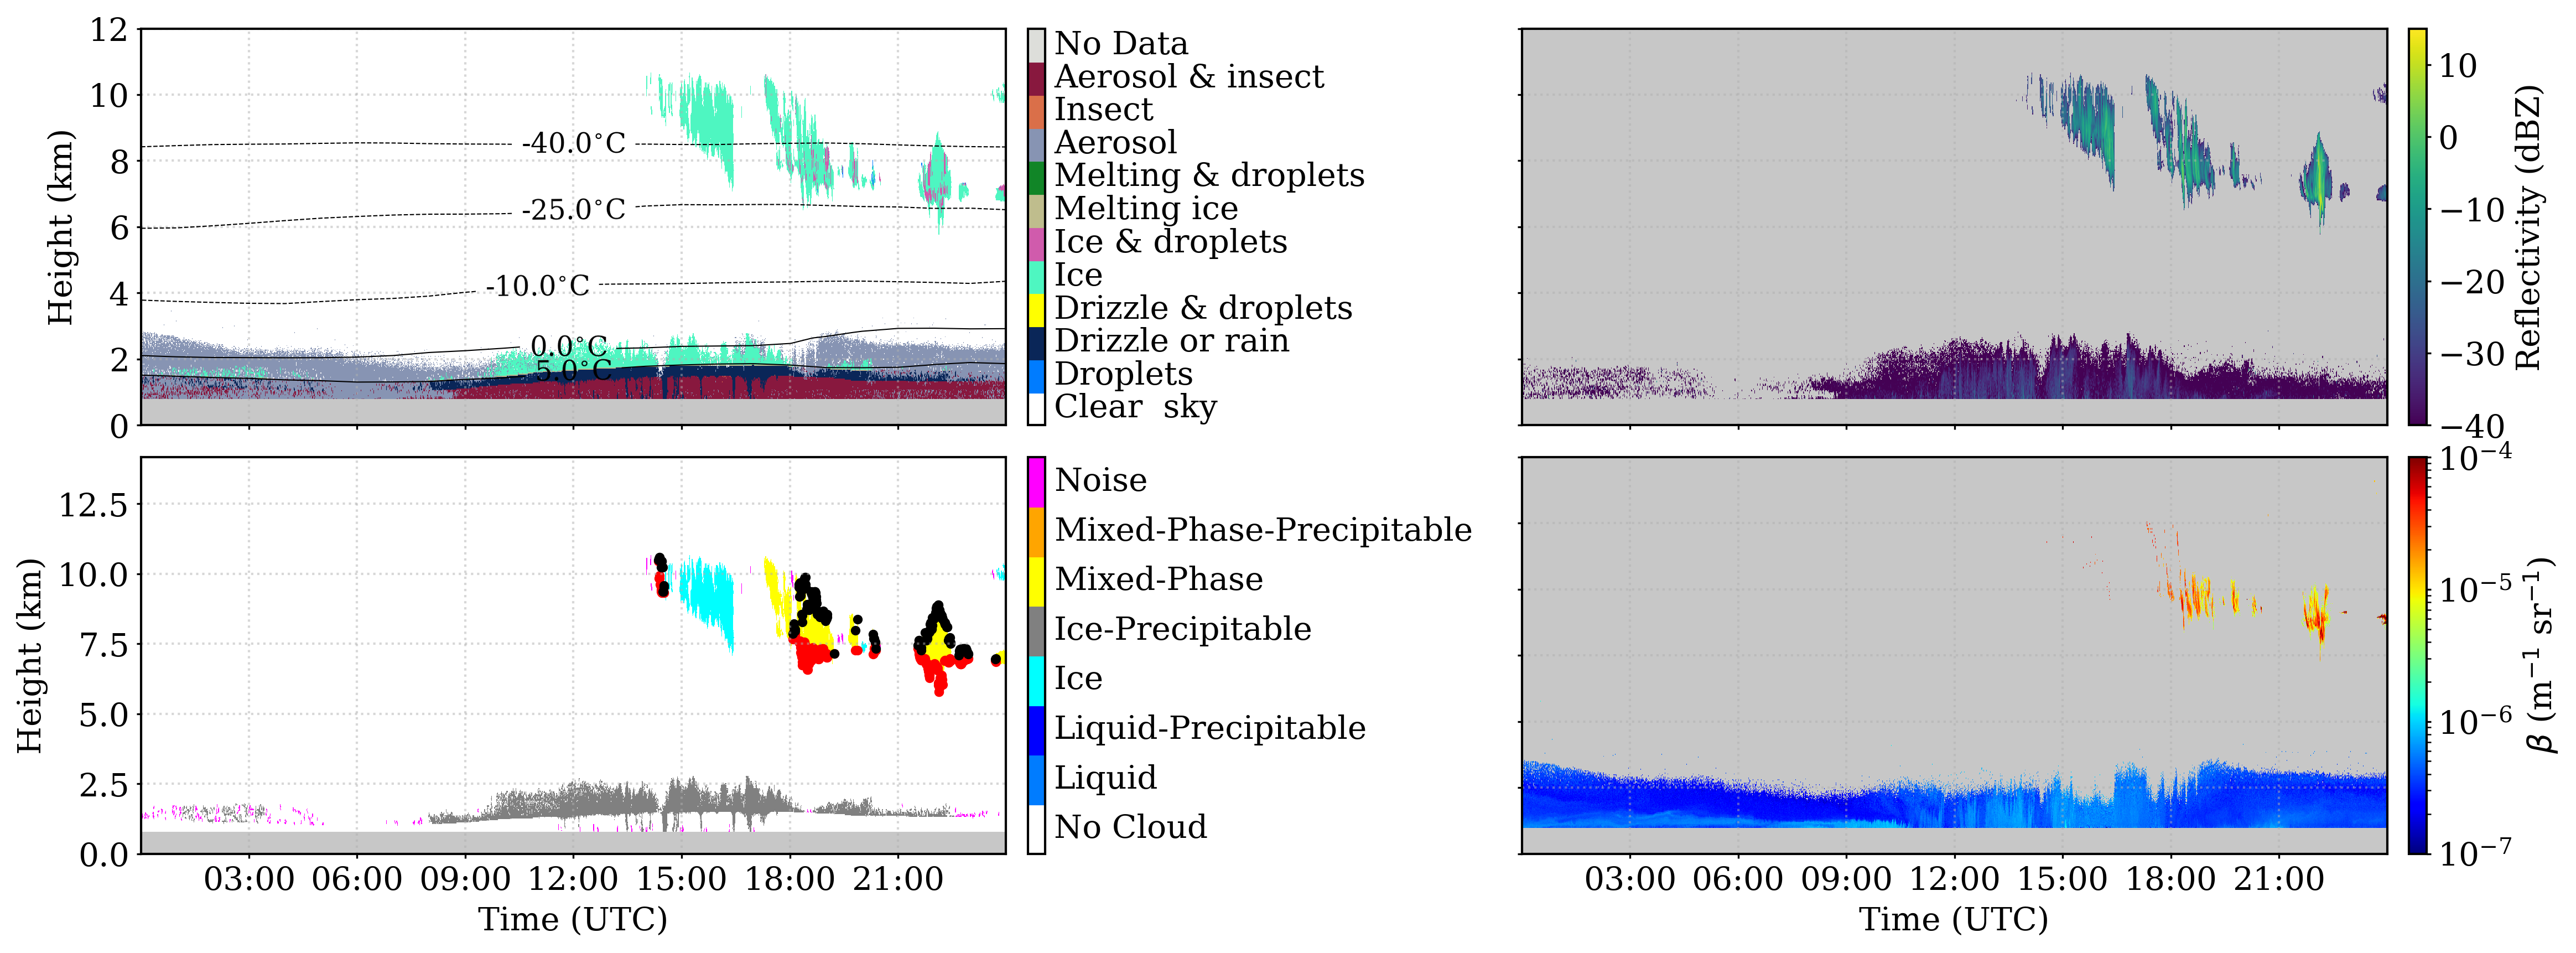
\includegraphics[width=\textwidth]{../../phd_clouds/figures/20210418_cloudnet_misclassification}
	\caption{A case study of Cloudnet hydrometeor misclassification. (a) Target classification product; (b) Radar reflectivity factor from Doppler cloud radar; (c) Attenuated backscattering coefficient from ceilometer. No evidence of clouds in the ABL can be identified by the instruments.}
	\label{fig:cloudnet_misclassification}
\end{figure}

Once the data are curated, the different cloud types are identified. Recent studies employed a cloud classification algorithm by profile with the aim of classify clouds
\citep{razvanpirloagaGroundBasedMeasurementsCloud2022, tatiananomokonovaStatisticsCloudsTheir2019, stefankneifelMultiyearCloudPrecipitation2021} and analyze their statistics. However, this algorithm admits different cloud typing inside the same cloud as a whole, assigning similar physical properties for different clouds. In the appendix \ref{sec:old_method}, we describe this algorithm, adapting the criteria used by \cite{razvanpirloagaGroundBasedMeasurementsCloud2022, tatiananomokonovaStatisticsCloudsTheir2019}.  
In this study we propose a new methodology to overcome these inaccuracies. We define a cloud as a group of at least 100 pixels identified by Cloudnet as droplet, drizzle (see Figure 3). To do so, a cloud mask is generated from the CLOUDNET target classification. Cloud pixels separated only by two pixels in any direction (analogous to 1 min, and 20 - 50 m of height) are considered part of the same cloud. This is achieved using a pixel dilation and contraction technique \citep{doughertyMathematicalMorphologyImage2018}, which expands and contracts the cloud shapes (see Appendix \ref{sec:dilation} for an explanation of the method). Once the cloud pixels are grouped, each cloud must have more than 100 pixels to be considered (without considering rain such as Drizzle or Rain pixels). Otherwise, it is deemed as an unknown type (likely noise). In order to illustrate this method, the left panel of Figure \ref{fig:cluster_identification} shows cloud clusters of different colors during an entire day (on 11 February 2021). The regions identified as clouds are marked by the black dashed lines in the right panel of the same figure, where clusters that are very close will merge to form one cloud. Also, small and isolated groups with less than 100 pixels are indicated by the red dashed lines

\begin{figure}[H]
	\centering
	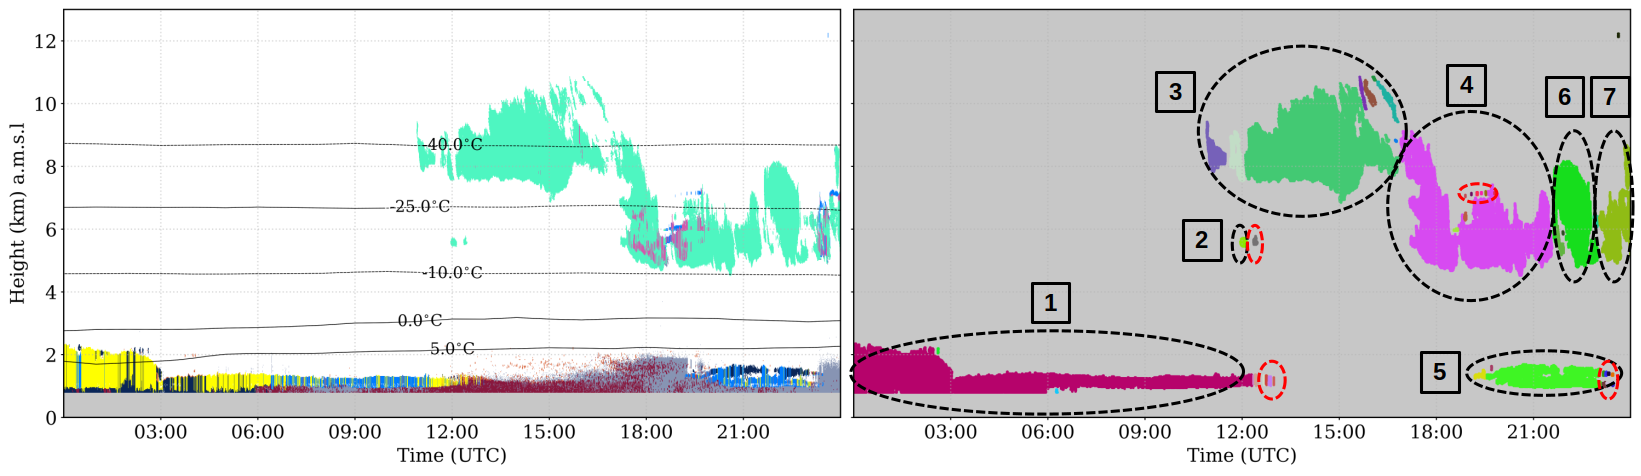
\includegraphics[width=.85\textwidth]{../../phd_clouds/figures/scheme_cloud_identification}
	\caption{Cloud cluster identification by Cloudnet target classification on 11 February 2021. (a) All hydrometeor clusters identified at different colors; (b) Cloud clusters identified in black dashed lines and noise by red dashed red}
	\label{fig:cluster_identification}
\end{figure}

Then, clouds are classified in six types: liquid, ice, mixed-phase, precipitating liquid, precipitating ice, and precipitating mixed-phase. To do so, the hydrometeor type percentages are calculated for each cloud, (shown in figure \ref{fig:classificationby_group_scheme}). A cloud is classified as liquid cloud (Liquid criteria) it comprises more than 70\% of Droplets and Drizzle plus Droplets. Then, it is further classified as a precipitating liquid cloud (Rainy criteria) if it contains at least 10 connected rain pixels, Similarly, a cloud is classified as an ice cloud (Ice criteria) if the previous verification is not satisfied and if  this group contains more than 90\% of ice or less than 10\% of Droplets plus Ice \& droplets. The same rain verification as in the liquid case is made to classify this group as a pure ice cloud or a precipitating ice cloud. Otherwise, clouds are classified as mixed-phase or precipitating mixed-phase through the same rain verification as in the other clouds.
In relation to precipitating ice and precipitating mixed-phase clouds, an extensive analysis of individual case studies revealed that Drizzle \& droplets only appear below the melting layer together with Drizzle \& rain droplets. Therefore, to avoid an underestimation of cloud base height due to drizzle, we removed these pixels for these clouds since they are probably rain.

\begin{figure}[H]
	\centering
	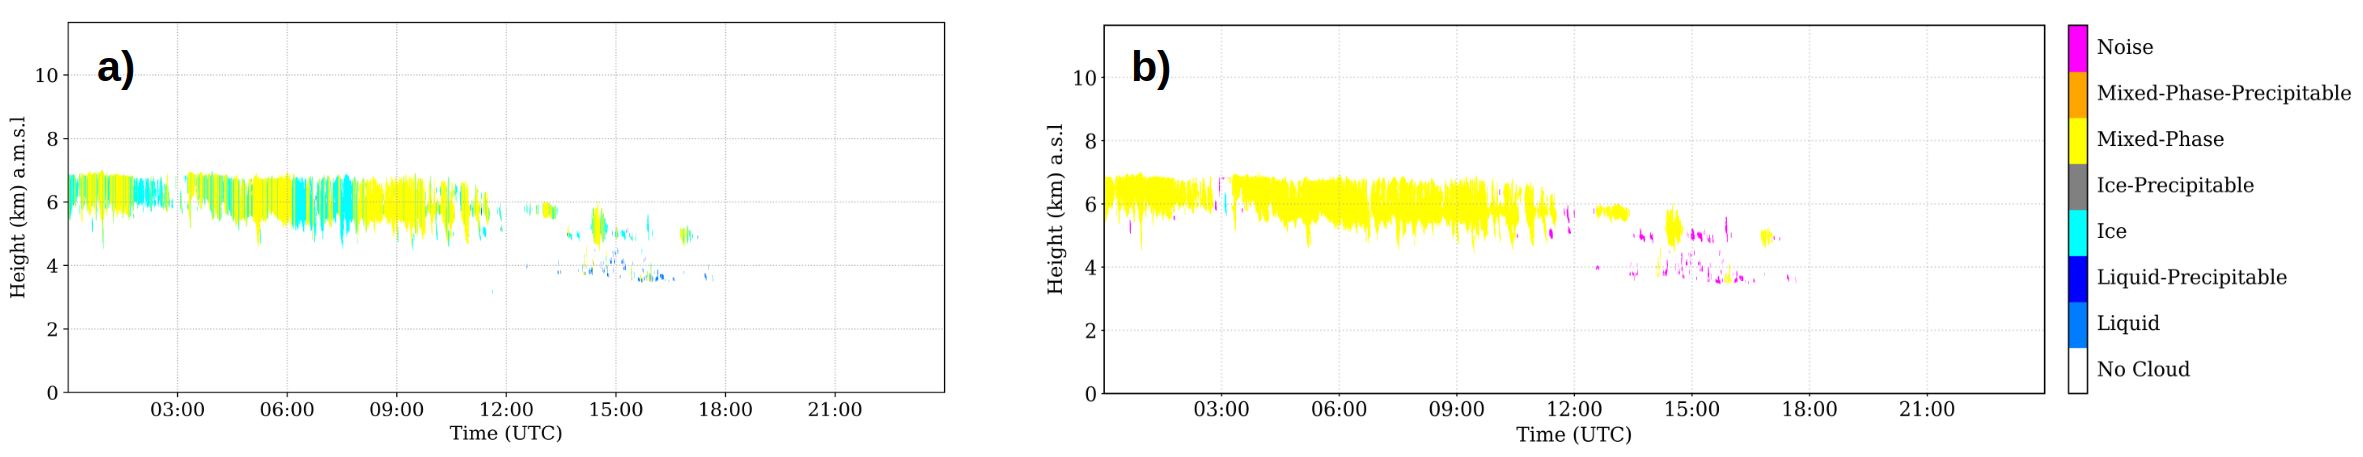
\includegraphics[width=.9\textwidth]{../../phd_clouds/figures/scheme_cloud_classification}
	\caption{Scheme of the cloud classification algorithm by hydrometeor grouping}
	\label{fig:classificationby_group_scheme}
\end{figure}

After the cloud classification, each cloud is then classified as single or multi-layer over time. Initially, time intervals where clouds overlap are identified. Overleaped pieces of clouds are classified as multi-layer, whereas non-overlapping pieces in principle are classified as single layer.We then analyzed cloud profiles for each cloud individually, acknowledging that a cloud can exhibit multiple layers with itself. If a cloud had a second layer separated by only one pixel at some time interval, that interval is identified as containing multi-layer. Otherwise, the clouds at that interval are classified as a single layer. 

In this study, only single layer clouds are analyzed. For the single layer case, cloud properties are calculated as follows: the cloud base and top height are determined by the first and last height pixels within the cloud layer, respectively. Cloud thickness is obtained by the difference between cloud base and top height pixels. 

\subsection{Cloud typing assessment}\label{sec:daily_cycle}

An evaluation of the classification algorithm presented in this study against the method used in the literature is conducted in order to evaluate its applicability for further analysis. Here, we aim to provide insights into the correlation on cloud statistics between different cloud categories generated by these two methods. In this framework, Figure \ref{fig:cloud_classification_comparison} shows a case study on 6 May of 2023 in Granada comparing profile-based cloud classification and cluster classification for a mixed phase cloud, where red and black dots represent the cloud base and top, respectively. As expected, the profile-based classification on the right panel leads to the fragmentation of a single cloud into different types. In this case, the same cloud is being classified as ice and mixed-phase by time. On the other hand, in the left panel, the new classification method preserves the homogeneity of the cloud and classifies it as mixed-phase cloud, resulting in a more realistic classification.

\begin{figure}[h]
	\centering
	\begin{subfigure}{0.48\textwidth}
		\centering
		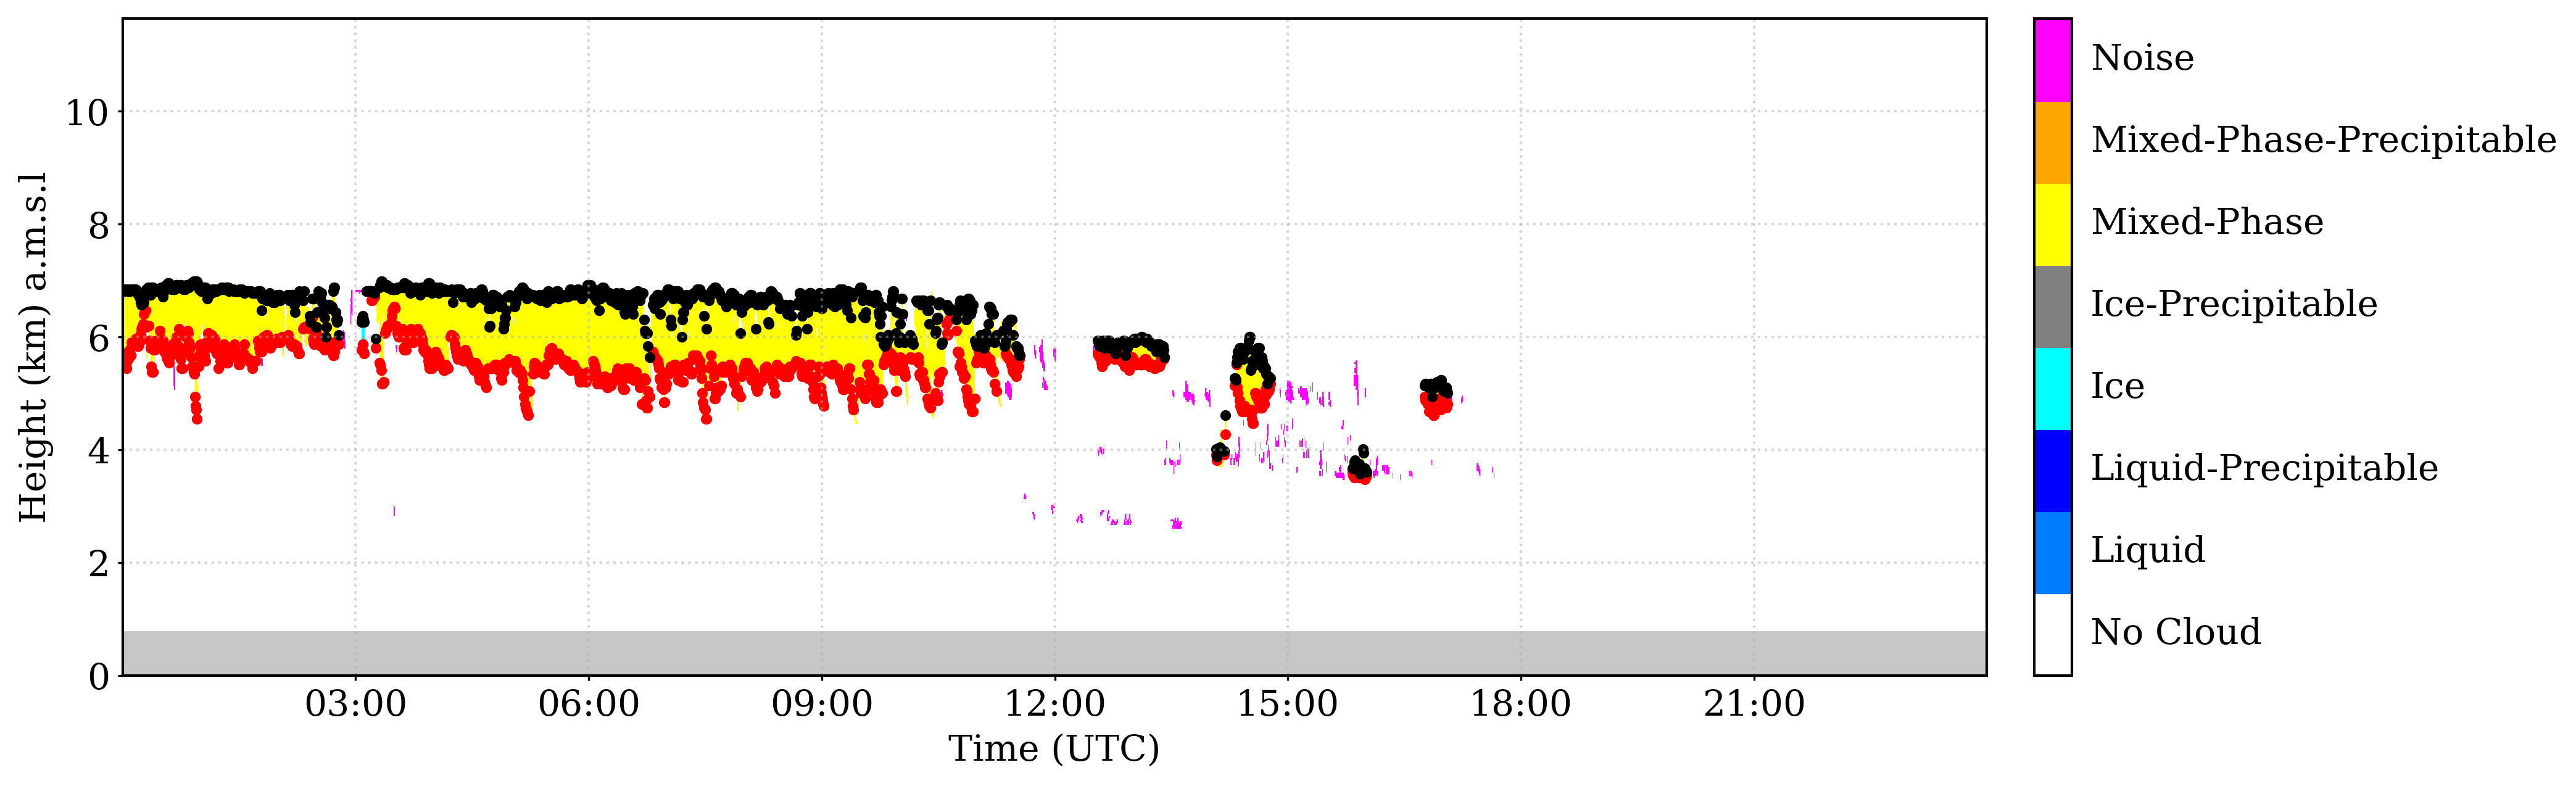
\includegraphics[width=\textwidth]{../../phd_clouds/figures/20230506_cloud_classification_new_method}
		\caption{Cloud classification using the new method.}
		\label{fig:new_method}
	\end{subfigure}
	\hfill
	\begin{subfigure}{0.48\textwidth}
		\centering
		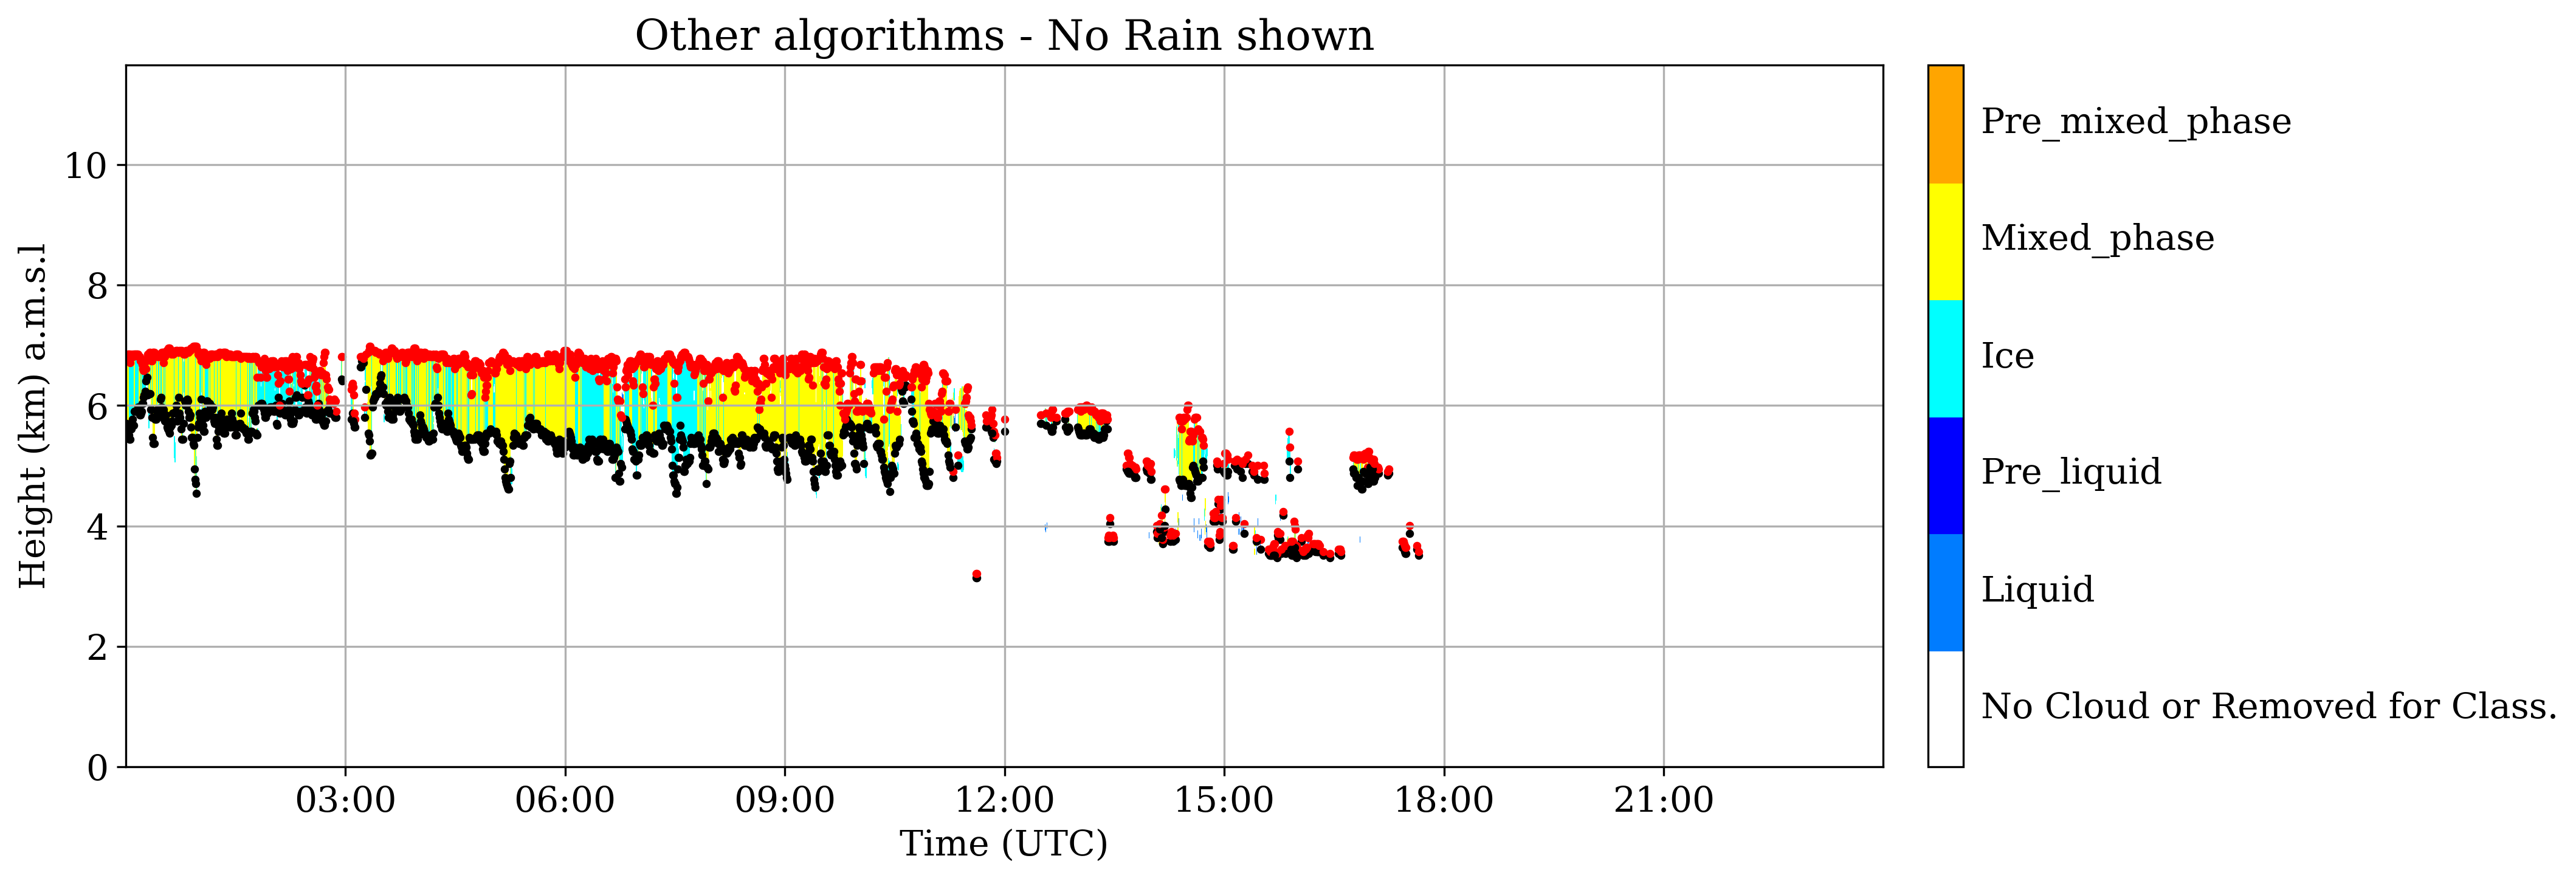
\includegraphics[width=\textwidth]{../../phd_clouds/figures/20230506_cloud_classification_old_method}
		\caption{Cloud classification using the old method.}
		\label{fig:old_method}
	\end{subfigure}
	\caption{Temporary figure (needs target classification). Comparison of cloud classification methods. The left panel illustrates the new method, which preserves cloud homogeneity and provides a more realistic classification. The right panel shows the old method used in recent studies, where cloud classification is time-based.}
	\label{fig:cloud_classification_comparison}
\end{figure}

As a consequence, the profile-based method of cloud classification can generate high correlations between cloud categories in terms of frequency of occurrence and cloud properties. Regarding cloud occurrence, the right panel of Figure~\ref{fig:cloud_classification_comparison} suggests that both ice and mixed phase clouds will have similar daily cloud occurrence and average cloud base. However, this is occurring because of the classification method, which could further affect cloud statistics.

Therefore, in order to quantify the correlation between cloud categories generated by these two classification algorithms, we calculate the daily cloud occurrence to assess the correlation between cloud types. Figure \ref{fig:pearson_correlation} shows the pearson correlation coefficients of daily cloud occurrence between cloud types for the cluster classification on the left, and for the classification by profile on the right. As it can be seen, the new proposed method demonstrates generally weaker correlations among cloud types, with most values clustering around zero. For example, the highest correlations observed were 0.19 between Liquid and Liquid-Precipitable clouds and 0.17 between Liquid and Mixed-Phase-Precipitable clouds, indicating relatively weak relationships. Additionally, some negligible negative correlations were observed, e.g. between Ice and Mixed-Phase-Precipitable clouds (-0.1). This suggests that the new method may provide a clearer distinction between cloud types, which is advantageous for analyses requiring precise classification. In contrast, the profile-based classification exhibited stronger and more pronounced correlations. Notably, the correlation between Ice and Mixed-Phase clouds was 0.4, and between Liquid and precipitating liquid clouds was 0.32, highlighting significant interdependencies between these cloud types. These relatively higher correlations are a consequence of the classification scheme defined in this method, which allows tagging multiple cloud types inside the same cloud domain. As a result, the comparison indicates that the new method, with its generally weaker correlations, may be better suited for distinguishing different cloud types. These findings underscore the importance of selecting an appropriate analytical method to study cloud properties between different cloud types.

\begin{figure}[H]
	\centering
	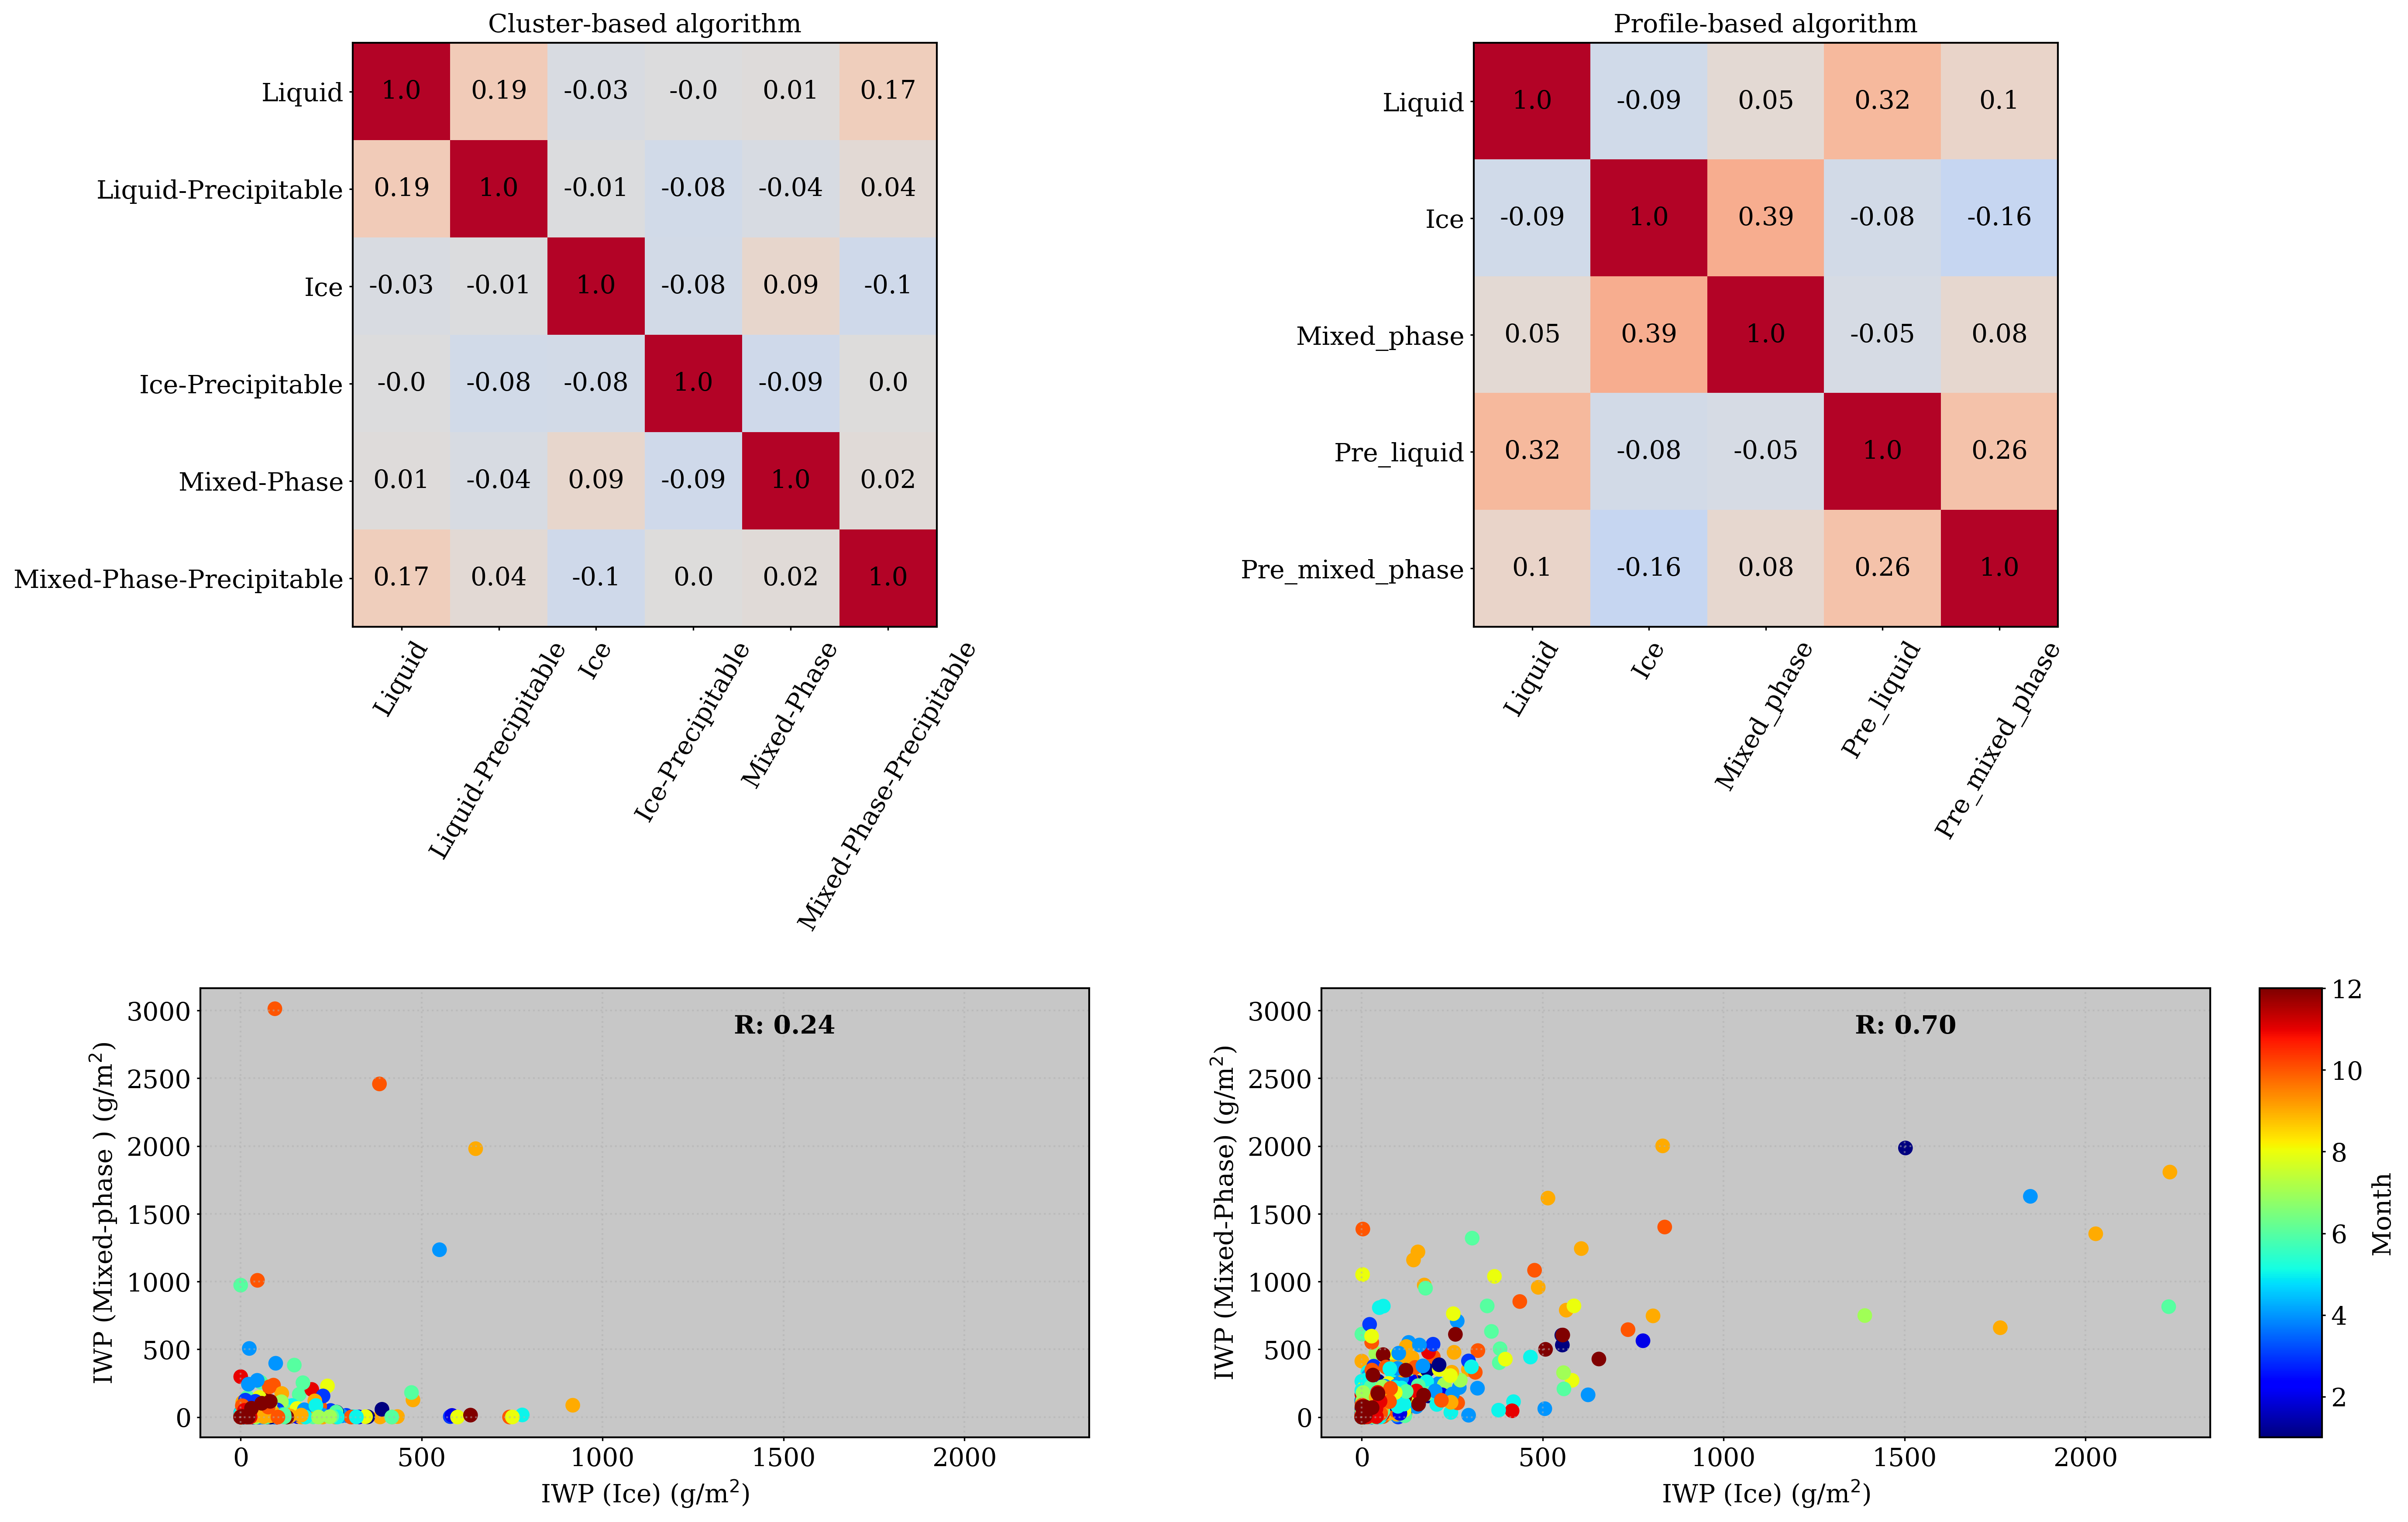
\includegraphics[width=.8\textwidth]{../../phd_clouds/figures/cloud_freq_methods_comparison_correlation_coefficient}
	\caption{The Pearson correlation matrix of daily cloud occurrence among different cloud types is shown in the top panel. The correlations for cluster-based methods are on the left and the profile-based correlation is on the right. Below each correlation matrix, the corresponding comparison of IWC between ice and mixed phase is shown.}
	\label{fig:pearson_correlation}
\end{figure}

Regarding the correlation in cloud properties, we computed the daily average of IWP for ice and mixed-phase clouds for the two classification methods. The bottom panel of Figure \ref{fig:pearson_correlation} shows the IWP of mixed phase clouds in function of the IWP of ice clouds. The R factor is the Pearson correlation coefficient between the IWP of these two cloud types. This coefficient is quite higher for the profile-based method, showing a correlation of 0.7. On the other hand, the cluster method exhibited only 0.24, with no apparent correlation. In addition, the correlation seems to be not monthly dependent as there is no clear separation by month. It is worthy to note that this section is not focused on the analysis of IWP, this will be done in section \ref{sec:cloud_microphys}. Instead of this, here we focused on the influence of the classification algorithm on cloud properties analysis. Following, the observations suggest that statistics on cloud properties can be highly influenced by the profile-based classification. As a result, this method may lead to the misinterpretation of real cloud properties, raising the relevance of previous evaluation of cloud classification algorithms before doing statistics on cloud properties. In this light, the new approach shows a promising classification method and will be employed in this study.


